\documentclass{standalone}

\usepackage{tikz}

\begin{document}

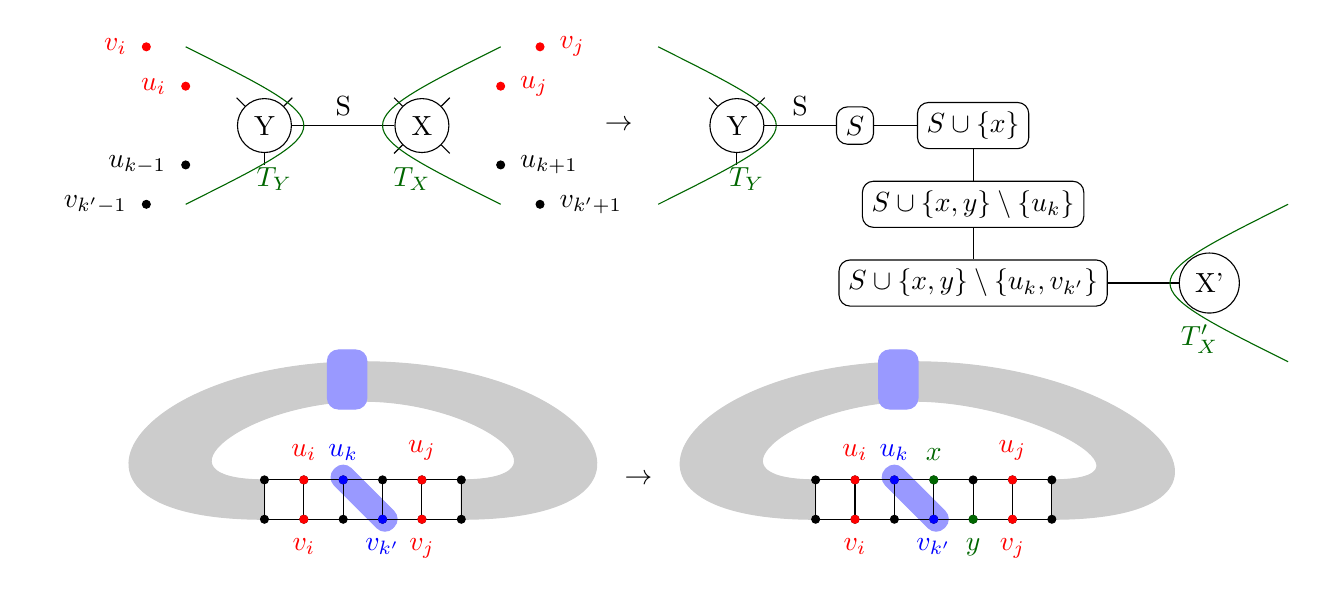
\begin{tikzpicture}
\def\radius{0.05}
\begin{scope}[shift={(-1,0)}]

% Main bags
\node[circle, draw] (Y) at (0,0) {Y};
\node[circle,draw] (X) at (2,0) {X};
% Points on the "left" side of S
%\draw[fill,blue] (-0.5,0) circle (\radius);
%\node[label={left:\textcolor{blue}{$a$}}] (a) at (-0.5,0) {};
\draw[fill] (-1.5,-1) circle (\radius);
\node[label={left:$v_{k'-1}$}] (a) at (-1.5,-1) {};
\draw[fill] (-1,-0.5) circle (\radius);
\node[label={left:$u_{k-1}$}] (a) at (-1,-0.5) {};
\draw[fill,red] (-1,0.5) circle (\radius);
\node[label={left:\textcolor{red}{$u_i$}}] (a) at (-1,0.5) {};
\draw[fill,red] (-1.5,1) circle (\radius);
\node[label={left:\textcolor{red}{$v_i$}}] (a) at (-1.5,1) {};
% Points to the "right" side of S
\draw[fill] (3.5,-1) circle (\radius);
\node[label={right:$v_{k'+1}$}] (a) at (3.5,-1) {};
\draw[fill] (3,-0.5) circle (\radius);
\node[label={right:$u_{k+1}$}] (a) at (3,-0.5) {};
\draw[fill,red] (3,0.5) circle (\radius);
\node[label={right:\textcolor{red}{$u_j$}}] (a) at (3,0.5) {};
\draw[fill,red] (3.5,1) circle (\radius);
\node[label={right:\textcolor{red}{$v_j$}}] (a) at (3.5,1) {};
%\draw[fill, blue] (2.5,0) circle (\radius);
%\node[label={right:\textcolor{blue}{$b$}}] (b) at (2.5,0) {};
% Tree dec edges (or sketches of tree dec edges)
\draw (X) -- node[midway, above] {S} (Y);
\draw (Y) -- +(45:0.5);
\draw (Y) -- +(135:0.5);
\draw (Y) -- +(-90:0.5);
\draw (X) -- +(-45:0.5);
\draw (X) -- +(-135:0.5);
\draw (X) -- +(45:0.5);
\draw (X) -- +(135:0.5);
\node (arrow) at (4.5,0) {$\rightarrow$};
\draw[green!40!black] (3,1) .. controls +(-2,-1) and +(-2,1) .. node[near end, below] {$T_X$} (3,-1);
\draw[green!40!black] (-1,1) .. controls +(2,-1) and +(2,1) .. node[near end, below] {$T_Y$} (-1,-1);
\end{scope}

\begin{scope}[shift={(5,0)}]

\node[circle, draw] (Y) at (0,0) {Y};
\draw (Y) -- +(45:0.5);
\draw (Y) -- +(135:0.5);
\draw (Y) -- +(-90:0.5);
    \draw[green!40!black] (-1,1) .. controls +(2,-1) and +(2,1) .. node[near end, below] {$T_Y$} (-1,-1);
\node[rectangle, rounded corners,draw] (S) at (1.5,0) {$S$};
\node[rectangle, rounded corners,draw] (S2) at (3,0) {$S\cup \{x\}$};
        \node[rectangle, rounded corners,draw] (S3) at (3,-1) {$S\cup \{x,y\}\setminus\{u_k\}$};
        \node[rectangle, rounded corners,draw] (S4) at (3,-2) {$S\cup \{x,y\}\setminus\{u_k,v_{k'}\}$};

    \node[circle,draw] (Xp) at (6,-2) {X'};
\draw (S) -- node[midway, above] {S} (Y);
\draw (S) --  (S2);
\draw (S2) --  (S3);
\draw (S3) --  (S4);
\draw (Xp) --  (S4);
        \draw[green!40!black] (7,-1) .. controls +(-2,-1) and +(-2,1) .. node[near end, below] {$T_{X}'$} (7,-3);
\end{scope}

    \begin{scope}[shift={(-1,-5)}]

\def\spacing{0.5}
\def\radius{0.05}

    \draw[rounded corners, fill, blue!40!white, rotate around={-45:(1.,0.25)}] (0.65,0.30) rectangle (1.7,0.6) ;
    
    \filldraw[black!20!white] (0,0) .. controls +(-3,0) and +(-3,0) .. (1.25,2) .. controls +(3,0) and +(3,0) .. (2.5,0) -- (2.5,0.5) .. controls +(1.5,0) and +(1.5,0) .. (1.25,1.5) .. controls +(-1.5,0) and +(-1.5,0) .. (0,0.5) -- cycle;
    \draw[rounded corners, fill, blue!40!white, rotate around={-90:(1.25,1.75)}] (0.85,1.30) rectangle (1.6,1.8) ;

%\node[label={left:\textcolor{blue}{$a$}}] (a) at (-1,1) {};
%\draw[fill, blue] (-1,1) circle (\radius);
%    \node[label={right:\textcolor{blue}{$b$}}] (b) at (3.5,1) {};
%\draw[fill, blue] (3.5,1) circle (\radius);

\foreach \i in {0,...,5}
{
    \draw[fill] (\i*\spacing,0) circle (\radius);
    \draw[fill] (\i*\spacing,\spacing) circle (\radius);
    \draw[fill] (\i*\spacing,0) -- (\i*\spacing,\spacing);
}

\foreach \i in {0,...,4}
{
    \draw[fill] (\i*\spacing,0) -- (\i*\spacing+\spacing,0);
    \draw[fill] (\i*\spacing,\spacing) -- (\i*\spacing+\spacing,\spacing);
}

\node[label={below:\textcolor{red}{$v_i$}}] (u) at (\spacing,0) {};
\node[label={above:\textcolor{red}{$u_i$}}] (u) at (\spacing,\spacing) {};
\draw[fill, red] (\spacing,0) circle (\radius);
\draw[fill, red] (\spacing,\spacing) circle (\radius);
\node[label={above:\textcolor{red}{$u_j$}}] (u) at (4*\spacing,\spacing) {};
\node[label={below:\textcolor{red}{$v_j$}}] (u) at (4*\spacing,0) {};
\draw[fill, red] (4*\spacing,\spacing) circle (\radius);
\draw[fill, red] (4*\spacing,0) circle (\radius);
\node[label={below:\textcolor{blue}{$v_{k'}$}}] (u) at (3*\spacing,0) {};
\node[label={above:\textcolor{blue}{$u_k$}}] (u) at (2*\spacing,\spacing) {};
\draw[fill, blue] (2*\spacing,\spacing) circle (\radius);
\draw[fill, blue] (3*\spacing,0) circle (\radius);

\end{scope}
\node at (3.75,-4.5) {$\rightarrow$};
    \begin{scope}[shift={(6,-5)}]

\def\spacing{0.5}
\def\radius{0.05}

    \draw[rounded corners, fill, blue!40!white, rotate around={-45:(1.,0.25)}] (0.65,0.30) rectangle (1.7,0.6) ;
    
    \filldraw[black!20!white] (0,0) .. controls +(-3,0) and +(-3,0) .. (1.25,2) .. controls +(3,0) and +(3,0) .. (3,0) -- (3,0.5) .. controls +(1.5,0) and +(1.5,0) .. (1.25,1.5) .. controls +(-1.5,0) and +(-1.5,0) .. (0,0.5) -- cycle;
    \draw[rounded corners, fill, blue!40!white, rotate around={-90:(1.25,1.75)}] (0.85,1.30) rectangle (1.6,1.8) ;

%\node[label={left:\textcolor{blue}{$a$}}] (a) at (-1,1) {};
%\draw[fill, blue] (-1,1) circle (\radius);
%    \node[label={right:\textcolor{blue}{$b$}}] (b) at (3.5,1) {};
%\draw[fill, blue] (3.5,1) circle (\radius);

\foreach \i in {0,...,6}
{
    \draw[fill] (\i*\spacing,0) circle (\radius);
    \draw[fill] (\i*\spacing,\spacing) circle (\radius);
    \draw[fill] (\i*\spacing,0) -- (\i*\spacing,\spacing);
}

\foreach \i in {0,...,5}
{
    \draw[fill] (\i*\spacing,0) -- (\i*\spacing+\spacing,0);
    \draw[fill] (\i*\spacing,\spacing) -- (\i*\spacing+\spacing,\spacing);
}

\node[label={below:\textcolor{red}{$v_i$}}] (u) at (\spacing,0) {};
\node[label={above:\textcolor{red}{$u_i$}}] (u) at (\spacing,\spacing) {};
\draw[fill, red] (\spacing,0) circle (\radius);
\draw[fill, red] (\spacing,\spacing) circle (\radius);
\node[label={above:\textcolor{red}{$u_j$}}] (u) at (5*\spacing,\spacing) {};
\node[label={below:\textcolor{red}{$v_j$}}] (u) at (5*\spacing,0) {};
\node[label={above:\textcolor{green!40!black}{$x$}}] (x) at (3*\spacing,\spacing) {};
\draw[fill, green!40!black] (4*\spacing,0) circle (\radius);
\draw[fill, green!40!black] (3*\spacing,\spacing) circle (\radius);
\node[label={below:\textcolor{green!40!black}{$y$}}] (y) at (4*\spacing,0) {};
\draw[fill, red] (5*\spacing,\spacing) circle (\radius);
\draw[fill, red] (5*\spacing,0) circle (\radius);
\draw[fill, blue] (2*\spacing,\spacing) circle (\radius);
\node[label={above:\textcolor{blue}{$u_k$}}] (u) at (2*\spacing,\spacing) {};
\draw[fill, blue] (3*\spacing,0) circle (\radius);
\node[label={below:\textcolor{blue}{$v_{k'}$}}] (u) at (3*\spacing,0) {};

\end{scope}

\end{tikzpicture}


\end{document}
